\chapter{Experimental Evaluation, Publication, and Maintenance}
\label{chapter:5_evaluation}

This Chapter reports the evaluation process of PEO. Sect. \ref{section:5_1_consistency} discusses the process of the ontology consistency check,
sect. \ref{section:5_2_ontometrics} measures ontology metrics , sect. \ref{section:5_3_oops} detects pitfall in PEO and sect. \ref{section:5_4_cqs} checks the execution of translated competency questions. In the final part of the chapter, sect. \ref{section:5_5_publication} discuss the publication and sect. \ref{section:5_6_discussion} discusses results obtained during the experimental evaluation.

\section{Ontology Consistency Check}
\label{section:5_1_consistency}
The ontology consistency check is a reasoning task available in OWL, and consequently Protege, that assesses the consistency of the ABox with respect to the TBox.
Hence, we execute the reasoner available in Protege that performs such check as well as other reasoning services including the rule-based inference.
We specifically adopt the HermiT reasoner.
Moreover, we consider both the manually populated and the automatic populate ontology.
On the original version of the PEO, the reasoner does not give any inconsistency and all the axioms are inferred correctly.
\begin{figure}[H]
    \centering
    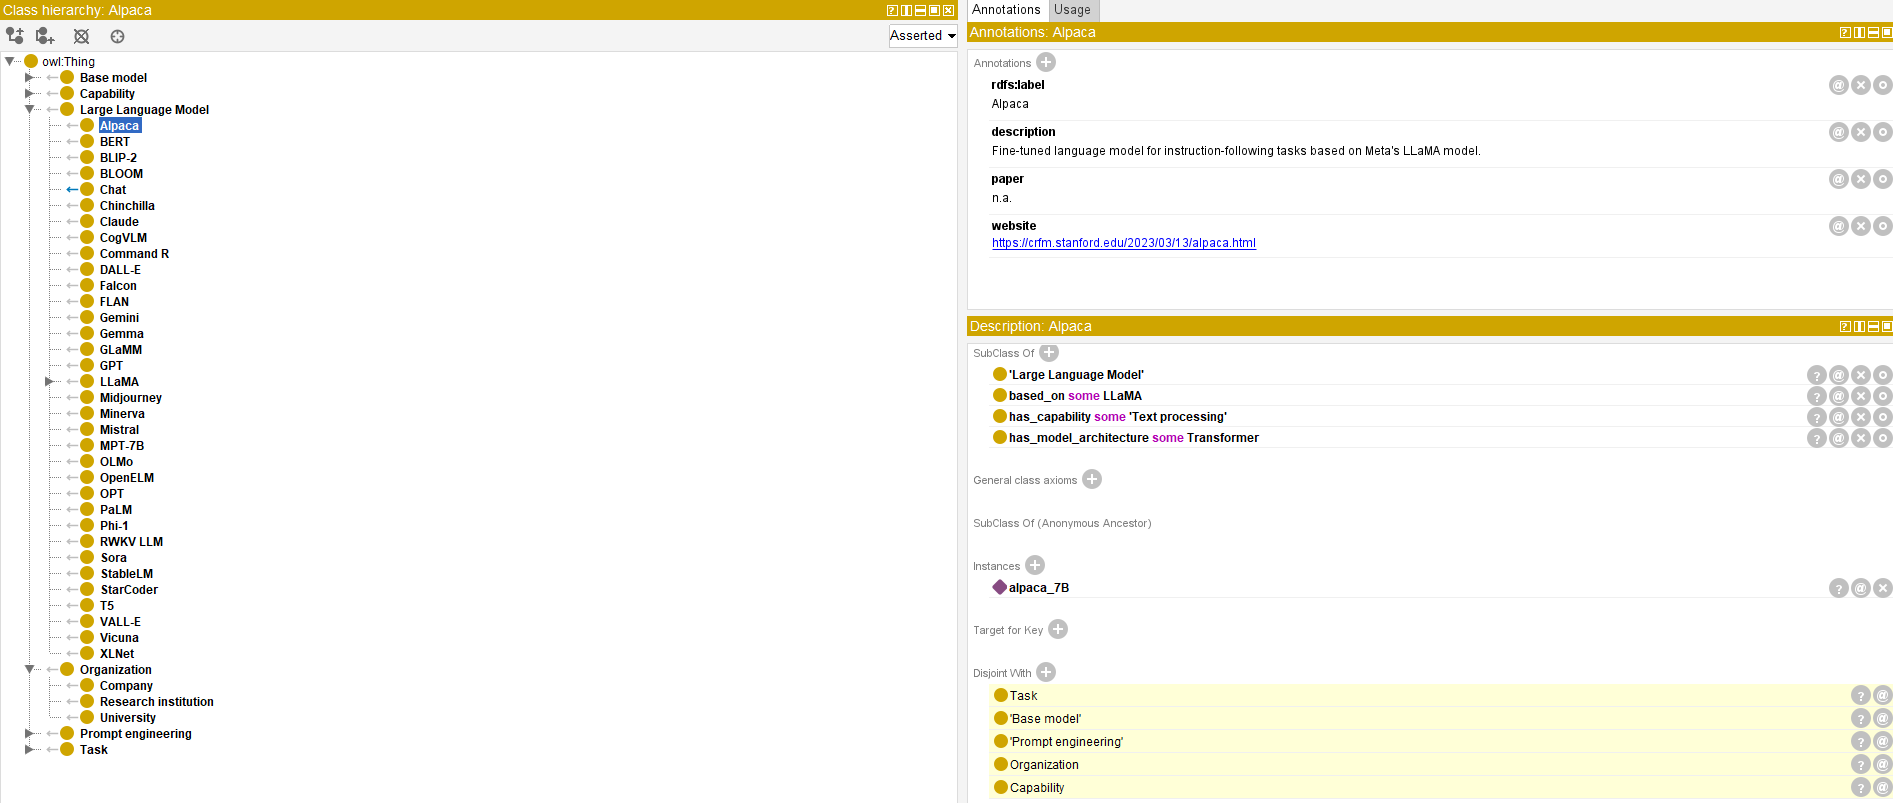
\includegraphics[width=0.9\linewidth]{Figures/fig_39.png}
    \caption{PEO with HermiT reasoner}
    \label{fig:39}
\end{figure}
Fig. \ref{fig:39} shows the execution of HermiT reasoner on PEO.
The reasoner infers correctly that the class "Alpaca" is disjoint with the classes "Task", "Base model", "Prompt engineering", "Organization" and "Capability" because the superclass "Large language model" is declared disjoint with that list of classes.
The ten SWRL rules declared work properly and infer the correct object properties for individuals:
\begin{figure}[H]
    \centering
    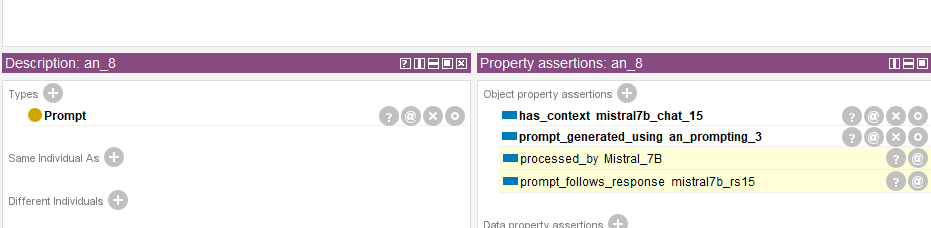
\includegraphics[width=0.9\linewidth]{Figures/fig_40.png}
    \caption{Inference on prompt individual}
    \label{fig:40}
\end{figure}
The consistency check of the other version of the PEO, the one populated using GPT-4 has given the exact results,  because as said in the previous section no additional significant information has been added to the ontology.
The classes added by GPT-4 have no link with the other existing classes and thus they do not lead to new inferences.

\section{OntoMetrics}
\label{section:5_2_ontometrics}
Moreover, we evaluated PEO based on OntoMetrics: a web-based tool developed by the University of Rostock that validates and provides statistical analyses of ontologies \cite{lantow2016ontometrics}.
Given the ontology in form of RDF file or code, it calculates automatically:
\begin{itemize}
    \item Base metrics: these include simple counts of ontology elements such as classes, axioms, and objects, providing a quantitative overview of the ontology's components.

    \item Schema Metrics: these metrics evaluate the structure of the ontology's schema, considering aspects like attribute richness and inheritance richness.

    \item Knowledge base Metrics: these assess the ontology's knowledge base, focusing on the population of instances within the ontology.

    \item Class Metrics: these metrics analyse individual classes within the ontology, examining factors such as class connectivity and fullness.

    \item Graph Metrics: these evaluate the ontology's taxonomy as a graph, measuring properties like depth and breadth.
\end{itemize}
For PEO, I will calculate base metrics, schema metrics and graph metrics.
\begin{figure}[H]
    \centering
    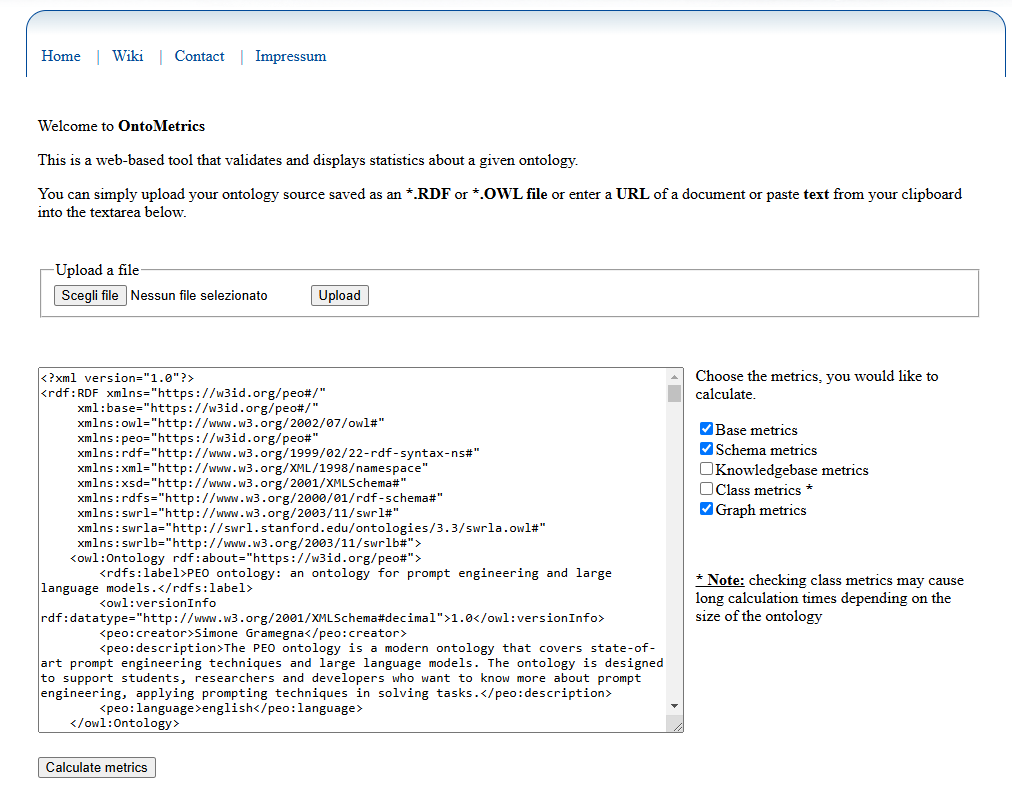
\includegraphics[width=0.9\linewidth]{Figures/fig_41.png}
    \caption{OntoMetrics interface}
    \label{fig:enter-label}
\end{figure}

The values computed for base metrics are reported in Tab.~\ref{tab:base_metrics_peo}.

\begin{table}[H]
    \footnotesize 
    \centering
    \begin{tabular}{|>{\raggedright\arraybackslash}p{8cm}|>{\raggedright\arraybackslash}p{4cm}|}
        \hline
        Property & Value \\ \hline
        Axioms & 2684 \\ \hline
        Logical axioms count & 1695 \\ \hline
        Class count & 126 \\ \hline
        Total classes count & 126 \\ \hline
        Object property count & 34 \\ \hline
        Total object properties count & 34 \\ \hline
        Data property count & 13 \\ \hline
        Total data properties count & 13 \\ \hline
        Properties count & 47 \\ \hline
        Individual count & 352 \\ \hline
        Total individuals count & 352 \\ \hline
        DL expressivity & SRIF(D) \\ \hline
    \end{tabular}
    \caption{PEO base metrics statistics}
    \label{tab:base_metrics_peo}
\end{table}
This table provides a high-level overview of the ontology’s structure and complexity.
With 2684 axioms, the ontology is rich in detail and represents a substantial body of knowledge.
Among these, 1695 logical axioms indicate a strong focus on enabling inference and reasoning.
The 126 classes show that the ontology has a robust framework for organizing concepts, while 34 object properties and 13 data properties highlight the ontology’s emphasis on relationships over attribute-driven modelling.
The inclusion of 352 individuals suggests that the ontology is well-populated, demonstrating practical applicability.
The expressivity of $SRIF(D)$ indicates that the ontology supports features like inverse roles and data ranges, balancing computational efficiency with expressive capability.
This ontology is comprehensive, but may require optimization to handle its inherent complexity effectively.

\begin{table}[H]
    \footnotesize 
    \centering
    \begin{tabular}{|>{\raggedright\arraybackslash}p{8cm}|>{\raggedright\arraybackslash}p{4cm}|}
        \hline
        Class Axiom Type & Count \\ \hline
        SubClassOf axioms count & 199 \\ \hline
        Equivalent classes axioms count & 1 \\ \hline
        Disjoint classes axioms count & 3 \\ \hline
        GCICount & 0 \\ \hline
        HiddenGCICount & 0 \\ \hline
    \end{tabular}
    \caption{PEO Class Axioms statistics}
    \label{tab:class-axioms_peo}
\end{table}
The table \ref{tab:class-axioms_peo} contains the count of the different class axiom types. 
There are one hundred ninety-nine SubClassOf axioms, there is just one Equivalent class axiom and there are three Disjoint classes axioms.
The Global Cardinality Restrictions count (GCICount) and Hidden Global Cardinality Restrictions count (HiddenGCICount) are both equal to zero. Those two indicators equal to zero mean that there are not explicit and implicit global cardinality restrictions.

\begin{table}[H]
    \footnotesize 
    \centering
    \begin{tabular}{|>{\raggedright\arraybackslash}p{8cm}|>{\raggedright\arraybackslash}p{4cm}|}
        \hline
        Object Property Axiom Type & Count \\ \hline
        SubObjectPropertyOf axioms count & 33 \\ \hline
        Equivalent object properties axioms count & 0 \\ \hline
        Inverse object properties axioms count & 16 \\ \hline
        Disjoint object properties axioms count & 0 \\ \hline
        Functional object properties axioms count & 0 \\ \hline
        Inverse functional object properties axioms count & 0 \\ \hline
        Transitive object property axioms count & 2 \\ \hline
        Symmetric object property axioms count & 0 \\ \hline
        Asymmetric object property axioms count & 0 \\ \hline
        Reflexive object property axioms count & 0 \\ \hline
        Irreflexive object property axioms count & 1 \\ \hline
        Object property domain axioms count & 33 \\ \hline
        Object property range axioms count & 33 \\ \hline
        SubPropertyChainOf axioms count & 0 \\ \hline
    \end{tabular}
    \caption{PEO Object Property Axioms Statistics}
    \label{tab:object-property-axioms_peo}
\end{table}
The table \ref{tab:object-property-axioms_peo} contains object property axiom types count in PEO.
There are thirty-three SubObjectPropertyOf axioms, while no Equivalent object properties or Disjoint object properties axioms are present. Additionally, the ontology includes 16 Inverse object properties axioms and two Transitive object property axioms.
Furthermore, no Functional, Inverse functional, Symmetric, or Asymmetric object property axioms are defined. There is also no Reflexive object property axiom, whereas one Irreflexive object property axiom is present.Regarding domain and range definitions, the ontology contains thirty-three Object property domain axioms and 33 Object property range axioms. Lastly, there are no SubPropertyChainOf axioms.


\begin{table}[H]
    \footnotesize 
    \centering
    \begin{tabular}{|>{\raggedright\arraybackslash}p{8cm}|>{\raggedright\arraybackslash}p{4cm}|}
        \hline
        Data Property Axiom Type & Count \\ \hline
        SubDataPropertyOf axioms count & 12 \\ \hline
        Equivalent data properties axioms count & 0 \\ \hline
        Disjoint data properties axioms count & 0 \\ \hline
        Functional data property axioms count & 7 \\ \hline
        Data property domain axioms count & 11 \\ \hline
        Data property range axioms count & 12 \\ \hline
    \end{tabular}
    \caption{PEO Data Property Axioms Statistics}
    \label{tab:data-property-axioms_peo}
\end{table}
Table \ref{tab:data-property-axioms_peo} presents the count of different data property axiom types in PEO. Specifically, there are twelve SubDataPropertyOf axioms, while no Equivalent data properties or Disjoint data properties axioms are present. Additionally, the ontology includes seven Functional data property axioms. Regarding domain and range definitions, the ontology contains eleven Data property domain axioms and twelve Data property range axioms.

\begin{table}[H]
    \footnotesize 
    \centering
    \begin{tabular}{|>{\raggedright\arraybackslash}p{8cm}|>{\raggedright\arraybackslash}p{4cm}|}
        \hline
        Individual Axiom Type & Count \\ \hline
        Class assertion axioms count & 352 \\ \hline
        Object property assertion axioms count & 390 \\ \hline
        Data property assertion axioms count & 580 \\ \hline
        Negative object property assertion axioms count & 0 \\ \hline
        Negative data property assertion axioms count & 0 \\ \hline
        Same individuals axioms count & 0 \\ \hline
        Different individuals axioms count & 0 \\ \hline
    \end{tabular}
    \caption{PEO Individual Axioms Statistics}
    \label{tab:individual-axioms_peo}
\end{table}
Table \ref{tab:individual-axioms_peo} presents the count of different individual axiom types in PEO. Specifically, there are three hundred fifty-two Class assertion axioms, three hundred ninety Object property assertion axioms, and five hundred eighty Data property assertion axioms. Additionally, there are no Negative object property assertion axioms, Negative data property assertion axioms, Same individuals axioms, or Different individuals axioms in the ontology.


\begin{table}[H]
    \footnotesize 
    \centering
    \begin{tabular}{|>{\raggedright\arraybackslash}p{8cm}|>{\raggedright\arraybackslash}p{4cm}|}
        \hline
        Annotation Axiom Type & Count \\ \hline
        Annotation axioms count & 5 \\ \hline
        Annotation assertion axioms count & 459 \\ \hline
        Annotation property domain axioms count & 0 \\ \hline
        Annotation property range axioms count & 0 \\ \hline
    \end{tabular}
    \caption{PEO Annotation Axioms Statistics}
    \label{tab:annotation-axioms_peo}
\end{table}
Table \ref{tab:annotation-axioms_peo} presents the count of different annotation axiom types in PEO. Specifically, there are five Annotation axioms and four hundred fifty-nine Annotation assertion axioms. Additionally, there are no Annotation property domain axioms or Annotation property range axioms in the ontology.


\begin{table}[H]
    \footnotesize 
    \centering
    \begin{tabular}{|>{\raggedright\arraybackslash}p{8cm}|>{\raggedright\arraybackslash}p{4cm}|}
        \hline
        Metric & Value \\ \hline
        Attribute richness & 0.103175 \\ \hline
        Inheritance richness & 1.579365 \\ \hline
        Relationship richness & 0.160338 \\ \hline
        Attribute class ratio & 0.0 \\ \hline
        Equivalence ratio & 0.007937 \\ \hline
        Axiom/class ratio & 21.301587 \\ \hline
        Inverse relations ratio & 0.390244 \\ \hline
        Class/relation ratio & 0.531646 \\ \hline
    \end{tabular}
    \caption{PEO Schema Metrics}
    \label{tab:ontology-metrics_peo}
\end{table}
Table \ref{tab:ontology-metrics_peo} presents the schema metrics for PEO. The Attribute richness is approximately zero point one, while the Inheritance richness is around one point six. The Relationship richness is about zero point one six. The Attribute class ratio is zero, and the Equivalence ratio is approximately zero point zero zero eight. The Axiom per class ratio is around twenty-one point three, whereas the Inverse relations ratio is about zero point three nine. Finally, the Class per relation ratio is approximately zero point five three.

\begin{table}[H]
    \footnotesize 
    \centering
    \begin{tabular}{|>{\raggedright\arraybackslash}p{8cm}|>{\raggedright\arraybackslash}p{4cm}|}
        \hline
        Metric & Value \\ \hline
        Absolute root cardinality & 7 \\ \hline
        Absolute leaf cardinality & 109 \\ \hline
        Absolute sibling cardinality & 126 \\ \hline
        Absolute depth & 318 \\ \hline
        Average depth & 2.52381 \\ \hline
        Maximal depth & 4 \\ \hline
        Absolute breadth & 126 \\ \hline
        Average breadth & 7.0 \\ \hline
        Maximal breadth & 33 \\ \hline
        Ratio of leaf fan-outness & 0.865079 \\ \hline
        Ratio of sibling fan-outness & 1.0 \\ \hline
        Tangledness & 0.269841 \\ \hline
        Total number of paths & 126 \\ \hline
        Average number of paths & 31.5 \\ \hline
    \end{tabular}
    \caption{PEO Graph Metrics}
    \label{tab:cardinality-depth-metrics_peo}
\end{table}
The table \ref{tab:cardinality-depth-metrics_peo}
The table \ref{tab:cardinality-depth-metrics_peo} provides graph metrics of PEO.
The absolute root cardinality (7) and absolute leaf cardinality (109) indicate a moderately deep hierarchy with good granularity at the leaf level.
The maximal depth (4) and average depth (2.52381) suggest a shallow graph, which can make the ontology easier to understand but may oversimplify complex domains.
The tangledness (0.269841) is moderate, indicating a graph structure that is connected but not overly complex.
The high sibling fan-out ratio (1.0) shows that sibling classes are evenly distributed, while the ratio of leaf fan-outness (0.865079) implies a balanced spread of subclasses from intermediate nodes.


Despite there being no significant differences between the original version of the PEO and the version populated using GPT-4, we proceed to calculate metrics.\\
Values computed for base metrics are:
\begin{table}[H]
    \footnotesize 
    \centering
    \begin{tabular}{|>{\raggedright\arraybackslash}p{8cm}|>{\raggedright\arraybackslash}p{4cm}|}
        \hline
        Property & Value \\ \hline
        Axioms & 2705 \\ \hline
        Logical axioms count & 1710 \\ \hline
        Class count & 128 \\ \hline
        Total classes count & 128 \\ \hline
        Object property count & 34 \\ \hline
        Total object properties count & 34 \\ \hline
        Data property count & 13 \\ \hline
        Total data properties count & 13 \\ \hline
        Properties count & 47 \\ \hline
        Individual count & 359 \\ \hline
        Total individuals count & 359 \\ \hline
        DL expressivity & SRIF(D) \\ \hline
    \end{tabular}
    \caption{PEO updated base metrics statistics}
    \label{tab:ontology-stats-updated}
\end{table}

\begin{table}[H]
    \footnotesize 
    \centering
    \begin{tabular}{|>{\raggedright\arraybackslash}p{8cm}|>{\raggedright\arraybackslash}p{4cm}|}
        \hline
        Class Axiom Type & Count \\ \hline
        SubClassOf axioms count & 197 \\ \hline
        Equivalent classes axioms count & 1 \\ \hline
        Disjoint classes axioms count & 3 \\ \hline
        GCICount & 0 \\ \hline
        HiddenGCICount & 0 \\ \hline
    \end{tabular}
    \caption{PEO updated Class Axioms Statistics}
    \label{tab:class-axioms-updated}
\end{table}

\begin{table}[H]
    \footnotesize 
    \centering
    \begin{tabular}{|>{\raggedright\arraybackslash}p{8cm}|>{\raggedright\arraybackslash}p{4cm}|}
        \hline
        Object Property Axiom Type & Count \\ \hline
        SubObjectPropertyOf axioms count & 33 \\ \hline
        Equivalent object properties axioms count & 0 \\ \hline
        Inverse object properties axioms count & 16 \\ \hline
        Disjoint object properties axioms count & 0 \\ \hline
        Functional object properties axioms count & 0 \\ \hline
        Inverse functional object properties axioms count & 0 \\ \hline
        Transitive object property axioms count & 8 \\ \hline
        Symmetric object property axioms count & 1 \\ \hline
        Asymmetric object property axioms count & 0 \\ \hline
        Reflexive object property axioms count & 0 \\ \hline
        Irreflexive object property axioms count & 1 \\ \hline
        Object property domain axioms count & 33 \\ \hline
        Object property range axioms count & 33 \\ \hline
        SubPropertyChainOf axioms count & 0 \\ \hline
    \end{tabular}
    \caption{PEO updated Object Property Axioms Statistics}
    \label{tab:object-property-axioms-updated}
\end{table}

\begin{table}[H]
    \footnotesize 
    \centering
    \begin{tabular}{|>{\raggedright\arraybackslash}p{8cm}|>{\raggedright\arraybackslash}p{4cm}|}
        \hline
        Data Property Axiom Type & Count \\ \hline
        SubDataPropertyOf axioms count & 12 \\ \hline
        Equivalent data properties axioms count & 0 \\ \hline
        Disjoint data properties axioms count & 0 \\ \hline
        Functional data property axioms count & 7 \\ \hline
        Data property domain axioms count & 12 \\ \hline
        Data property range axioms count & 12 \\ \hline
    \end{tabular}
    \caption{PEO updated Data Property Axioms Statistics}
    \label{tab:data-property-axioms-updated}
\end{table}

\begin{table}[H]
    \footnotesize 
    \centering
    \begin{tabular}{|>{\raggedright\arraybackslash}p{8cm}|>{\raggedright\arraybackslash}p{4cm}|}
        \hline
        Individual Axiom Type & Count \\ \hline
        Class assertion axioms count & 358 \\ \hline
        Object property assertion axioms count & 393 \\ \hline
        Data property assertion axioms count & 580 \\ \hline
        Negative object property assertion axioms count & 0 \\ \hline
        Negative data property assertion axioms count & 0 \\ \hline
        Same individuals axioms count & 0 \\ \hline
        Different individuals axioms count & 0 \\ \hline
    \end{tabular}
    \caption{PEO updated Individual Axioms Statistics}
    \label{tab:individual-axioms-updated}
\end{table}

\begin{table}[H]
    \footnotesize 
    \centering
    \begin{tabular}{|>{\raggedright\arraybackslash}p{8cm}|>{\raggedright\arraybackslash}p{4cm}|}
        \hline
        Annotation Axiom Type & Count \\ \hline
        Annotation axioms count & 5 \\ \hline
        Annotation assertion axioms count & 456 \\ \hline
        Annotation property domain axioms count & 0 \\ \hline
        Annotation property range axioms count & 0 \\ \hline
    \end{tabular}
    \caption{PEO updated Annotation Axioms Statistics}
    \label{tab:annotation-axioms-updated}
\end{table}

The schema metrics for the update version of PEO are:
\begin{table}[H]
    \footnotesize 
    \centering
    \begin{tabular}{|>{\raggedright\arraybackslash}p{8cm}|>{\raggedright\arraybackslash}p{4cm}|}
        \hline
        Metric & Value \\ \hline
        Attribute richness & 0.101563 \\ \hline
        Inheritance richness & 1.539063 \\ \hline
        Relationship richness & 0.161702 \\ \hline
        Attribute class ratio & 0.0 \\ \hline
        Equivalence ratio & 0.007813 \\ \hline
        Axiom/class ratio & 21.132813 \\ \hline
        Inverse relations ratio & 0.390244 \\ \hline
        Class/relation ratio & 0.544681 \\ \hline
    \end{tabular}
    \caption{PEO Schema Metrics}
    \label{tab:ontology-metrics-updated}
\end{table}

The graph metrics for updated version of PEO are:

\begin{table}[H]
    \footnotesize 
    \centering
    \begin{tabular}{|>{\raggedright\arraybackslash}p{8cm}|>{\raggedright\arraybackslash}p{4cm}|}
        \hline
        Metric & Value \\ \hline
        Absolute root cardinality & 11 \\ \hline
        Absolute leaf cardinality & 111 \\ \hline
        Absolute sibling cardinality & 128 \\ \hline
        Absolute depth & 316 \\ \hline
        Average depth & 2.46875 \\ \hline
        Maximal depth & 4 \\ \hline
        Absolute breadth & 128 \\ \hline
        Average breadth & 7.111111 \\ \hline
        Maximal breadth & 33 \\ \hline
        Ratio of leaf fan-outness & 0.867188 \\ \hline
        Ratio of sibling fan-outness & 1.0 \\ \hline
        Tangledness & 0.265625 \\ \hline
        Total number of paths & 128 \\ \hline
        Average number of paths & 32.0 \\ \hline
    \end{tabular}
    \caption{PEO updated Graph Metrics}
    \label{tab:cardinality-depth-metrics-updated}
\end{table}
The new values calculated by OntoMetrics on the updated version of the ontology do not differ significantly from the previously calculated values, as the large language model GPT-4 has only added four new classes and three new instances. All results for PEO and its second version are on Github \footnote{https://github.com/simonegramegna/peo/tree/main/evaluation}.
\section{Static Validation}
\label{section:5_3_oops}
The methods discussed so far are widely used in ontology evaluation; however, they are not capable of capturing modelling errors in greater detail. These errors can compromise not only the quality and usability of the ontology but also lead to potential inconsistencies. Therefore, it is necessary to adopt a different approach from those previously examined, OntoMetrics and the HermiT reasoner, because they have the following issues:
\begin{itemize}
    \item OntoMetrics: it provides a quantitative measure of ontology's structural characteristics without analysing qualitative aspects, so it is not able to detect semantic
    issues in the ontology.

    \item HermiT reasoner (reasoners in general): reasoners are designed to check the logical consistency of an ontology and perform inferencing identifying inconsistencies in axioms. But reasoners are not able to detect errors outside logical inconsistencies, such as missing domain or range definitions and they cannot check best-practice violation and usability issues.
\end{itemize}
These limitations highlight the need for a tool that can go beyond structural and logical evaluation, addressing both semantic and usability dimensions of ontology quality.
OOPS! (Ontology Pitfall Scanner) is an online tool for ontology evaluation \cite{poveda2014oops} that automates the evaluation process without requiring any effort by the developer. 
\begin{figure}[H]
    \centering
    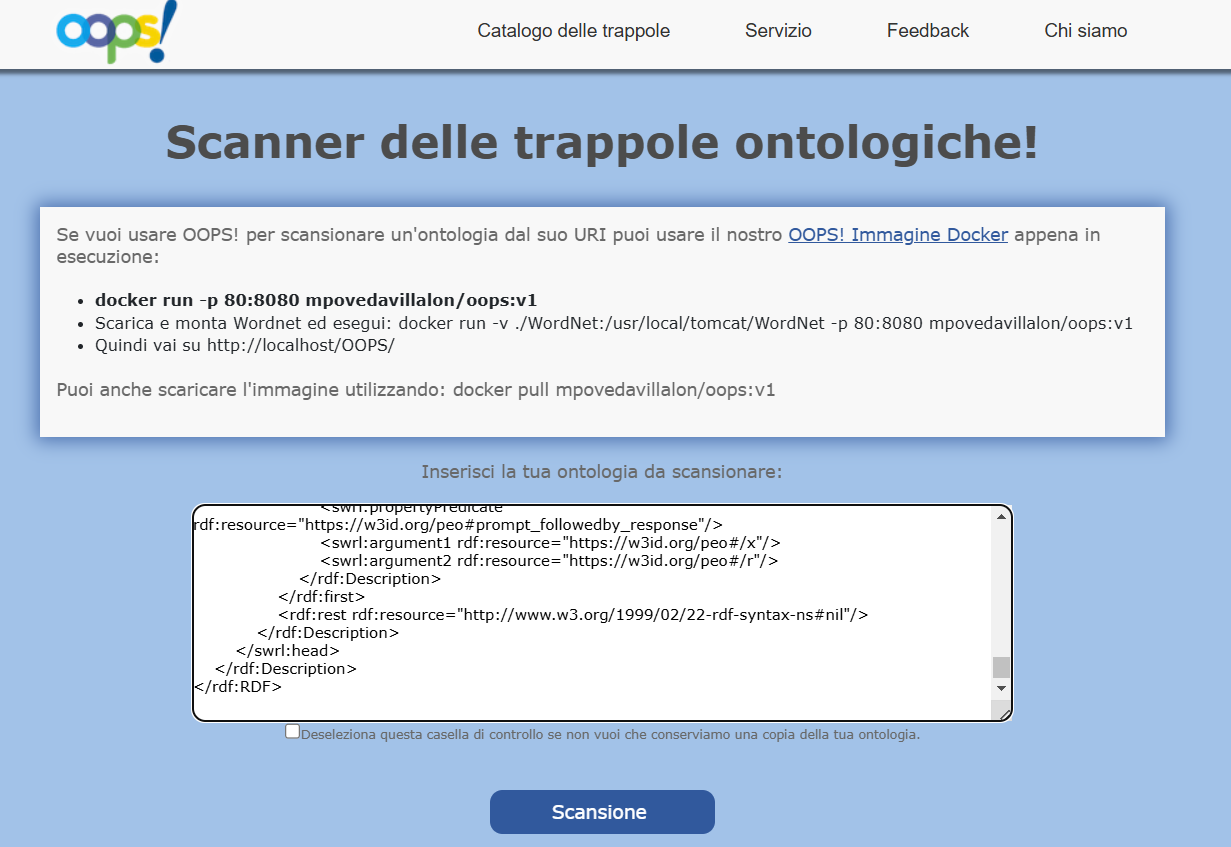
\includegraphics[width=0.9\linewidth]{Figures/fig_42.png}
    \caption{OOPS! web interface}
    \label{fig:42}
\end{figure}
Fig \ref{fig:42} shows the oops web interface.
Given the input ontology, OOPS is able to detect 40 different pitfall that are classified into three categories: critical, important and minor by parsing the RDF code and generating a complete response using the OOPS! scanner. Pitfalls in the scanner include:
\begin{itemize}
    \item Structural pitfalls: formal structure and syntax like cycles in hierarchy and unconnected ontology elements.

    \item Functional pitfalls: use and functionality of the ontology like missing domain or incorrectly defined inverse relationships.

    \item Usability and Profiling Pitfalls: clarity, maintainability, and human-readability like missing annotations, inconsistent naming and ambiguous terms.
\end{itemize}
I will use OOPS! scanner on both versions of the PEO detecting and explaining found pitfalls. 
For the first version of PEO there are just three pitfalls:
\begin{figure}[H]
    \centering
    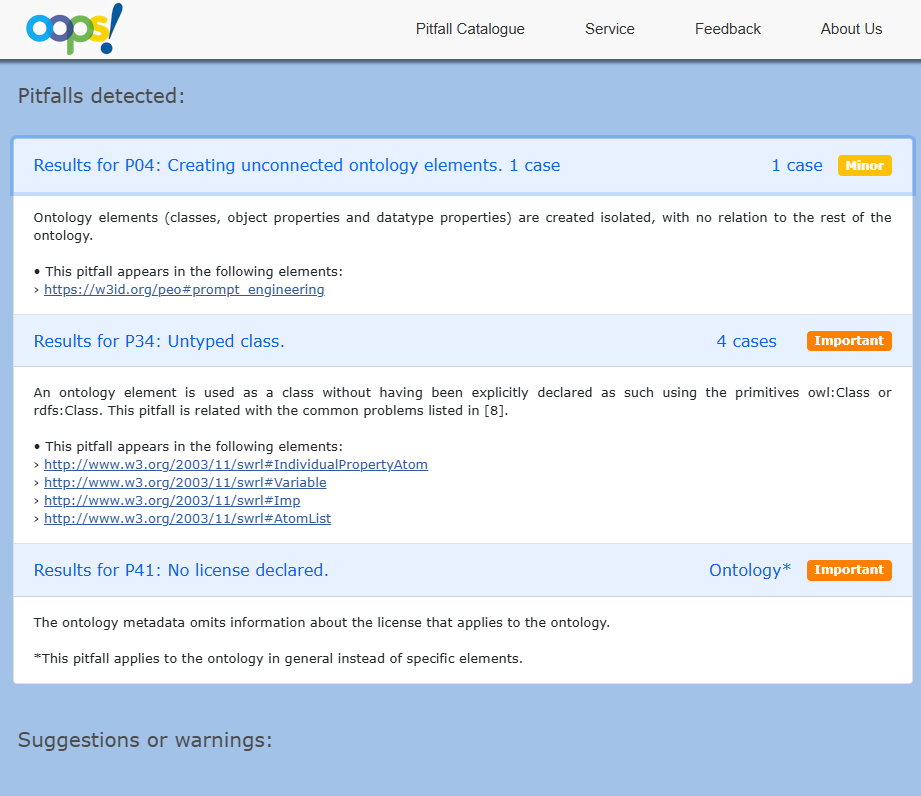
\includegraphics[width=0.9\linewidth]{Figures/fig_43.png}
    \caption{Detected pitfalls PEO}
    \label{fig:enter-label}
\end{figure}
The explanation of detected pitfall is:
\begin{itemize}
    \item P04 (Creating unconnected ontology elements): this pitfall involves ontology elements (classes, object properties and datatype properties) are created isolated, with no relation to the rest of the ontology. 

    \item P34 (Untyped class): this pitfalls involves all ontology elements that are used as a class without having explicitly declared. This pitfall involves four elements in PEO: \\ http://www.w3.org/2003/11/swrl\#IndividualPropertyAtom,\\ http://www.w3.org/2003/11/swrl\#Variable,\\ http://www.w3.org/2003/11/swrl\#Imp and \\http://www.w3.org/2003/11/swrl\#AtomList.

    \item P41 (No license declared): there is no license in the ontology metadata.    
\end{itemize}
Overall, the report is satisfactory, as no critical pitfalls have been identified, nor any issues found in the main classes or object properties of the ontology and I will discuss in more detail in Results discussion section.
The complete report is available here \footnote{https://github.com/simonegramegna/peo/blob/main/evaluation/oops\_report\_peo.xml}. After detecting pitfalls in the original version of the PEO, I also examined the populated version generated using GPT-4 nonetheless, no significant differences were observed between the two versions. Compared to the three pitfalls identified in the previous version, OOPS detects five pitfalls:
\begin{figure}[H]
    \centering
    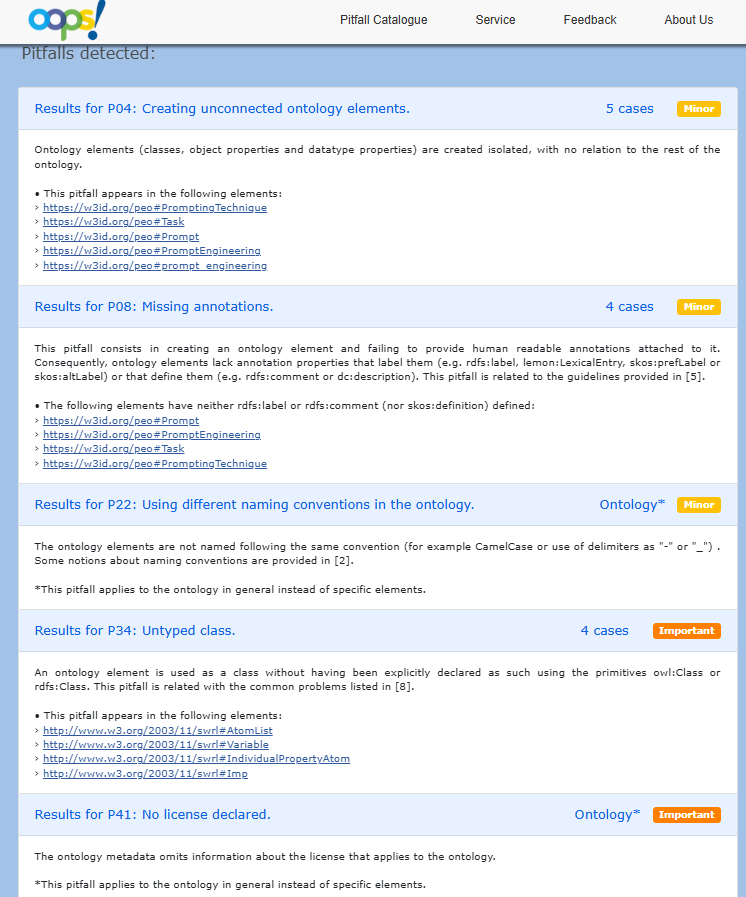
\includegraphics[width=0.75\linewidth]{Figures/fig_44.png}
    \caption{Detected pitfalls second version PEO}
    \label{fig:enter-label}
\end{figure}


\begin{itemize}
    \item P04 (Creating unconnected ontology elements): this pitfall, as said before, involves unconnected ontology elements. This time the pitfall involves not only the prompt\_engineering class but also the new classes created by GPT-4: Task, PromptingTechnique, Prompt and PromptEngineering. Those classes have no relations with other classes.

    \item P08 (Missing annotations): this pitfall involves elements that lack annotation properties that label them ( rdfs:label) or that define them\\ (rdfs:comment). This pitall involves the four classes created by GPT-4 with no comment provided: Task, PromptingTechnique, Prompt and PromptEngineering.  

    \item P22 (Using different naming conventions in the ontology): this pitfall involves ontology elements are not named following the same convention (for example CamelCase or use of delimiters as "-" or "\_"). This pitfall is given by the new classes created by GPT-4 that do not follow the naming convention used in the ontology (with the "\_" separator) by creating classes declared in camel case.

    \item P34 (Untyped class): this is the same pitfall detected before.

    \item P41 (No license declared): this is the same pitfall detected before.
\end{itemize}
In general, the detected pitfalls are caused by GPT-4's lack of understanding of the ontology's structure and I will discuss in more detail in the Results discussion section. The oops report is available here \footnote{https://github.com/simonegramegna/peo/blob/main/evaluation/oops_report_peo_gpt4.xml}.


\section{Competency Questions}
\label{section:5_4_cqs}
The final step of ontology evaluation is converting the CQs defined in the Ontology requirements specification section into SPARQL queries in order to compare the expected result to the actual result of each CQ.
SPARQL queries are generated manually and executed using Jupyter notebook \footnote{https://jupyter.org/}: an enviroment for running python code and the rdflib python library rdflib \footnote{https://rdflib.readthedocs.io/en/stable/}: a library to access rdf files and run SPARQL queries inside python.
The code is available in the  Github repository  \footnote{https://github.com/simonegramegna/peo/tree/main/evaluation}.
The evaluation is mode for both versions of the ontology.\\
Firstly, the ontology is loaded with rdflib as represented in fig. \ref{fig:45}
\begin{figure}[H]
    \centering
    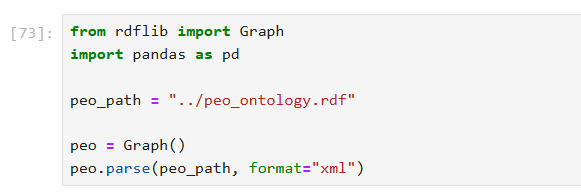
\includegraphics[width=0.9\linewidth]{Figures/fig_45.png}
    \caption{Jupyter notebook SPARQL}
    \label{fig:45}
\end{figure}
The pandas library is used to display query results in data-frames.
For such purpose, we implemented three helper functions:
\begin{itemize}
    \item execute\_query: it takes as input the SPARQL query string and returns a list of results.

    \item results\_to\_df: it takes as input as input the list of results ad creates and returns a dataframe with results inside which columns' names are the label names.

    \item print\_results: it iterates on the list of results and prints each element.
\end{itemize}
We can see the implementation below, in fig. \ref{fig:46}:
\begin{figure}[H]
    \centering
    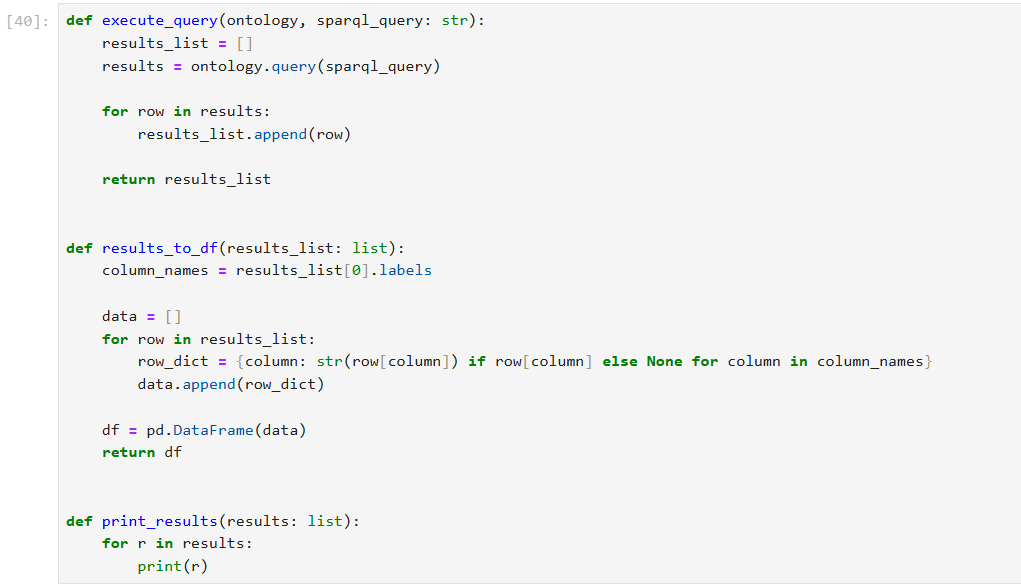
\includegraphics[width=0.9\linewidth]{Figures/fig_46.png}
    \caption{Support python functions}
    \label{fig:46}
\end{figure}

Once this is done, we can translate each of the sixteen CQs into SPARQL queries to be executed on PEO.\\
The first CQ CQ1: What is prompt engineering? is translated into:
\begin{lstlisting}
    SELECT DISTINCT ?property ?value
    WHERE {
        <https://w3id.org/peo#prompt_engineering> ?property ?value .
    }
\end{lstlisting}
\begin{figure}[H]
    \centering
    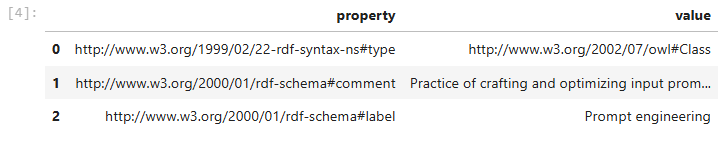
\includegraphics[width=0.9\linewidth]{Figures/fig_47.png}
    \caption{CQ1 SPARQL query results}
    \label{fig:47}
\end{figure}
The output, in fig. \ref{fig:47}, from the query matches the expected result, which is the definition of prompt engineering.\\

The second competency question CQ2: What is a prompt? is translated into:
\begin{lstlisting}
SELECT DISTINCT ?property ?value
WHERE {
    <https://w3id.org/peo#prompt> ?property ?value .
}
\end{lstlisting}
\begin{figure}[H]
    \centering
    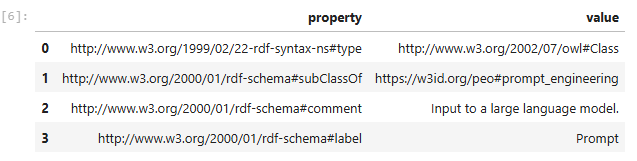
\includegraphics[width=0.9\linewidth]{Figures/fig_48.png}
    \caption{CQ2 SPARQL query results}
    \label{fig:48}
\end{figure}

The output, in fig. \ref{fig:48}, also in this case matches the expected result, which is the definition of prompt.\\

The third competency question CQ3: What are prompting techniques? is translated into:
\begin{lstlisting}
SELECT DISTINCT ?subclass ?label
WHERE {
    ?subclass rdfs:subClassOf <https://w3id.org/peo#prompting_technique> .
    OPTIONAL { ?subclass rdfs:label ?label . }
}
\end{lstlisting}

\begin{figure}[H]
    \centering
    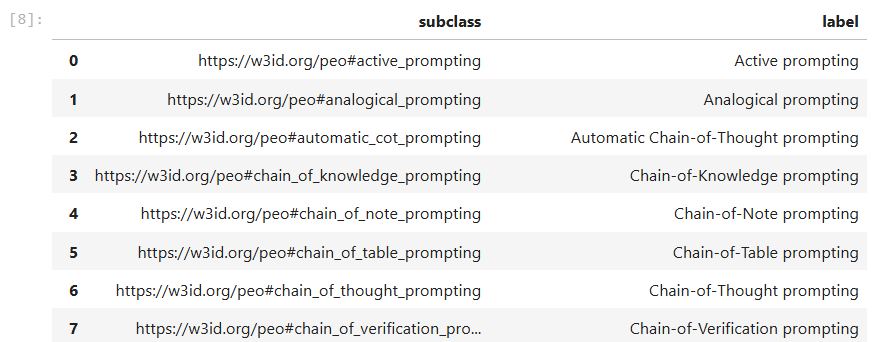
\includegraphics[width=0.9\linewidth]{Figures/fig_49.png}
    \caption{CQ3 SPARQL query results}
    \label{fig:49}
\end{figure}
The complete table contains, in fig. \ref{fig:49}, all the prompting techniques in the ontology.\\

The fourth competency question CQ4: What are image prompting techniques? is translated into:
\begin{lstlisting}
SELECT DISTINCT ?subclass ?label
WHERE {
    ?subclass rdfs:subClassOf <https://w3id.org/peo#image_prompting> .
    OPTIONAL { ?subclass rdfs:label ?label . }
}
\end{lstlisting}

\begin{figure}[H]
    \centering
    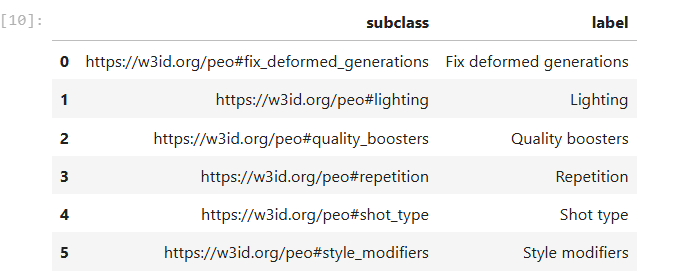
\includegraphics[width=0.9\linewidth]{Figures/fig_50.png}
    \caption{CQ4 SPARQL query results}
    \label{fig:50}
\end{figure}
As expected. in fig \ref{fig:50}, we get all the image prompting techniques in the ontology.\\

The fifth competency question CQ5: What are code prompting techniques? is translated into:
\begin{lstlisting}
SELECT DISTINCT ?subclass ?label
WHERE {
    ?subclass rdfs:subClassOf <https://w3id.org/peo#code_prompting> .
    OPTIONAL { ?subclass rdfs:label ?label . }
}  
\end{lstlisting}

\begin{figure}[H]
    \centering
    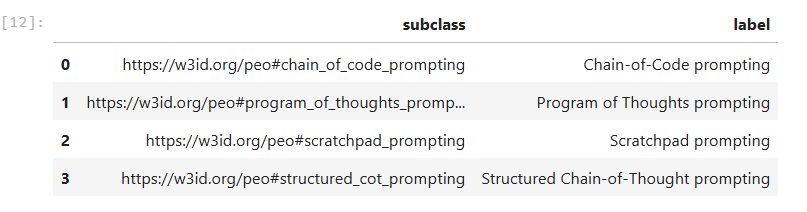
\includegraphics[width=0.9\linewidth]{Figures/fig_51.png}
    \caption{CQ5 SPARQL query results}
    \label{fig:51}
\end{figure}
The table contains, in \ref{fig:51}, all the code prompting techniques in the ontology.\\

The sixth competency question CQ6: Which task does a prompt solve? is translated into:
\begin{lstlisting}
SELECT DISTINCT ?prompt ?task ?taskLabel
WHERE {
    ?prompt <https://w3id.org/peo#solves> ?task .
    OPTIONAL { ?task rdfs:label ?taskLabel . }
}
\end{lstlisting}

\begin{figure}[H]
    \centering
    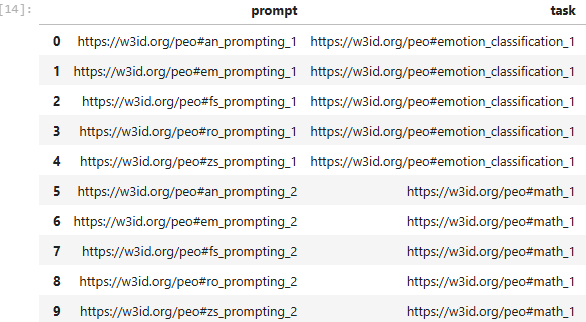
\includegraphics[width=0.9\linewidth]{Figures/fig_52.png}
    \caption{CQ6 SPARQL query results}
    \label{fig:52}
\end{figure}
The table contains, in fig \ref{fig:52}, all the prompts that solve tasks.\\

The seventh competency question CQ7: Which prompts are generated using a prompting technique? is translated into:
\begin{lstlisting}
SELECT DISTINCT ?prompt ?technique ?techniqueLabel
WHERE {
    ?prompt <https://w3id.org/peo#prompt_generated_using> ?technique .
    OPTIONAL { ?technique rdfs:label ?techniqueLabel . }
}
\end{lstlisting}

\begin{figure}[H]
    \centering
    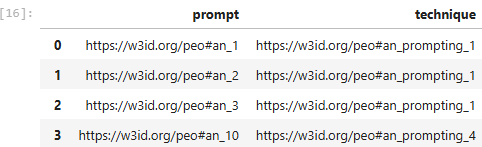
\includegraphics[width=0.9\linewidth]{Figures/fig_53.png}
    \caption{CQ7 SPARQL query results}
    \label{fig:53}
\end{figure}
The complete table, in fig \ref{fig:53}, contains all the prompt instances generated using instances of prompting techniques.\\

The eighth competency question CQ8: What are the responses that follow each prompt? is translated into:
\begin{lstlisting}
SELECT DISTINCT ?prompt ?response
WHERE {
    ?response <https://w3id.org/peo#response_followedby_prompt> ?prompt .
}    
\end{lstlisting}

\begin{figure}[H]
    \centering
    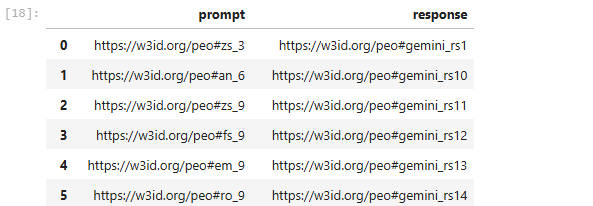
\includegraphics[width=0.9\linewidth]{Figures/fig_54.png}
    \caption{CQ8 SPARQL query results}
    \label{fig:54}
\end{figure}
The complete table contains, in fig. \ref{fig:54}, all the responses of all prompt instances.\\

The ninth competency question CQ9: What are possible tasks? is translated into:
\begin{lstlisting}
SELECT DISTINCT ?task ?label
WHERE {
    ?task rdf:type owl:Class .
    ?task rdfs:subClassOf* <https://w3id.org/peo#task> .
    OPTIONAL { ?task rdfs:label ?label . }
}    
\end{lstlisting}

\begin{figure}[H]
    \centering
    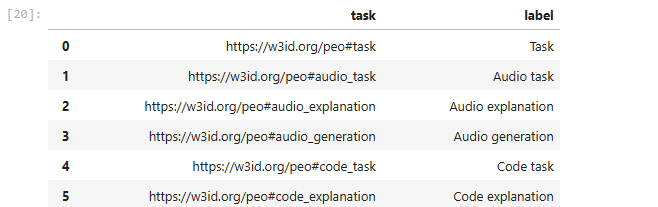
\includegraphics[width=0.9\linewidth]{Figures/fig_55.png}
    \caption{CQ9 SPARQL query results}
    \label{fig:55}
\end{figure}
In the completed table, in \ref{fig:55}, we get all the possible task represented in the ontology.\\

The tenth competency question CQ10: Which tasks are related to the text? is translated into:
\begin{lstlisting}
SELECT DISTINCT ?task ?label
WHERE {
    ?task rdf:type owl:Class .
    ?task rdfs:subClassOf* <https://w3id.org/peo#text_task> .
    OPTIONAL { ?task rdfs:label ?label . }
}
\end{lstlisting}

\begin{figure}[H]
    \centering
    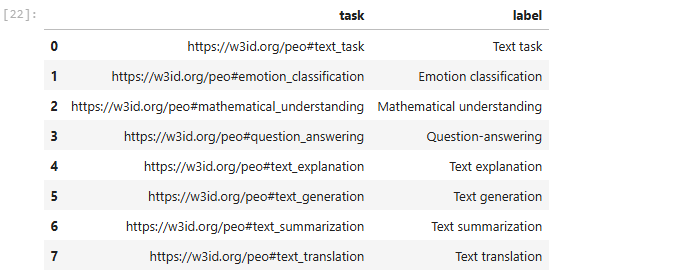
\includegraphics[width=0.9\linewidth]{Figures/fig_56.png}
    \caption{CQ10 SPARQL query results}
    \label{fig:56}
\end{figure}

The resulting table, in fig. \ref{fig:56}, contains, all the task related to text.\\

The eleventh competency question CQ11: What is a chat? is translated into:
\begin{lstlisting}
SELECT DISTINCT ?property ?value
WHERE {
    <https://w3id.org/peo#chat> ?property ?value .
}
\end{lstlisting}

\begin{figure}[H]
    \centering
    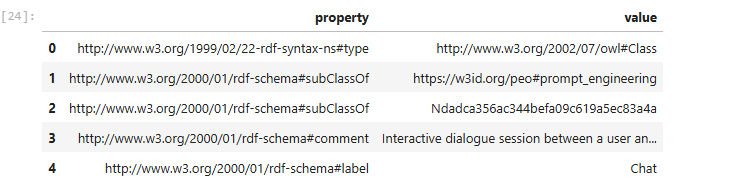
\includegraphics[width=0.9\linewidth]{Figures/fig_57.png}
    \caption{CQ11 SPARQL query results}
    \label{fig:57}
\end{figure}
The result, in fig. \ref{fig:57}, is the definition of Chat.\\

The twelfth competency question CQ12: What is a large language model? is translated into:
\begin{lstlisting}
SELECT DISTINCT ?property ?value
WHERE {
    <https://w3id.org/peo#large_language_model> ?property ?value .
}
\end{lstlisting}

\begin{figure}[H]
    \centering
    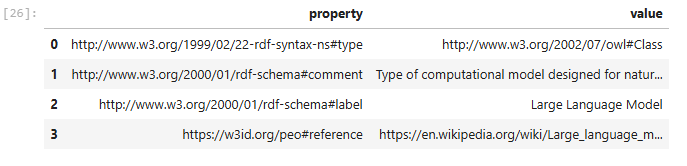
\includegraphics[width=0.9\linewidth]{Figures/fig_58.png}
    \caption{CQ12 SPARQL query results}
    \label{fig:58}
\end{figure}
The result, in fig \ref{fig:58}, is the definition of Large Language Model.\\

The thirteenth competency question CQ13: What types of large language models are available? is translated into:
\begin{lstlisting}
SELECT DISTINCT ?type ?label
WHERE {
    ?type rdfs:subClassOf <https://w3id.org/peo#large_language_model> .
    OPTIONAL { ?type rdfs:label ?label . }
}
\end{lstlisting}

\begin{figure}[H]
    \centering
    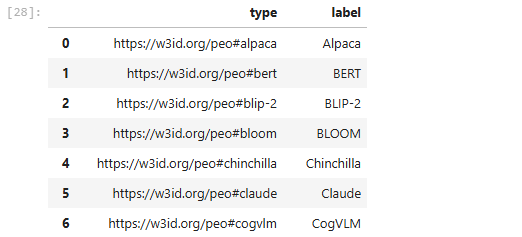
\includegraphics[width=0.9\linewidth]{Figures/fig_59.png}
    \caption{CQ13 SPARQL query results}
    \label{fig:59}
\end{figure}
The resulting complete table, in fig. \ref{fig:59}, is the collection of all large language models represented in the ontology.\\

The fourteenth competency question CQ14: What are large language models architectures? is translated into:
\begin{lstlisting}
SELECT DISTINCT ?type ?label
WHERE {
    ?type rdfs:subClassOf <https://w3id.org/peo#base_model> .
    OPTIONAL { ?type rdfs:label ?label . }
}   
\end{lstlisting}

\begin{figure}[H]
    \centering
    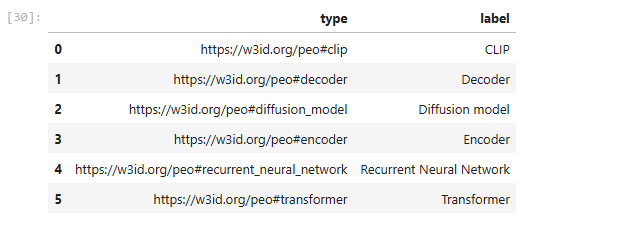
\includegraphics[width=0.9\linewidth]{Figures/fig_60.png}
    \caption{CQ14 SPARQL query results}
    \label{fig:60}
\end{figure}
The result, in fig. \ref{fig:60}, is the collection of main large language models architectures.\\

The fifteenth competency question CQ15: What are large language models capabilities? is translated into:
\begin{lstlisting}
SELECT DISTINCT ?type ?label
WHERE {
    ?type rdfs:subClassOf <https://w3id.org/peo#capability> .
    OPTIONAL { ?type rdfs:label ?label . }
}
\end{lstlisting}

\begin{figure}[H]
    \centering
    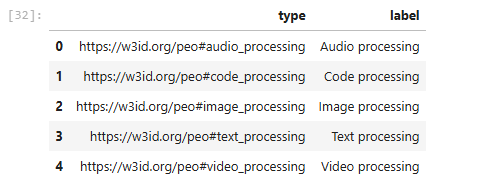
\includegraphics[width=0.8\linewidth]{Figures/fig_61.png}
    \caption{CQ15 SPARQL query results}
    \label{fig:61}
\end{figure}
Results are represented, in fig. \ref{fig:61}, by the collection of all the capabilities represented in PEO.\\

The sixteenth and last competency question CQ16: What companies develop large language models? is translated into:
\begin{lstlisting}
SELECT DISTINCT ?company ?label
WHERE {
    ?company rdf:type <https://w3id.org/peo#company> .
    OPTIONAL { ?company rdfs:label ?label . }
}
\end{lstlisting}

\begin{figure}[H]
    \centering
    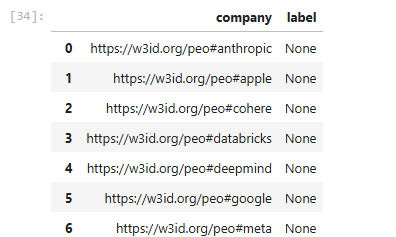
\includegraphics[width=0.8\linewidth]{Figures/fig_62.png}
    \caption{CQ16 SPARQL query results}
    \label{fig:62}
\end{figure}
The result, in fig. \ref{62}, is the collection of companies that develop large language models.\\
We proceed also, to execute SPARQL queries on the second version of PEO, the one that has been populated automatically using GPT-4. 
We translated only competency questions that match changes introduced by the LLM. Competency questions chosen for translation are four: CQ1, CQ2, CQ3 and CQ9.\\
The first competency question CQ1: What is prompt engineering? is translated into:
\begin{lstlisting}
SELECT DISTINCT ?property ?value
WHERE {
    <https://w3id.org/peo#PromptEngineering> ?property ?value .
} 
\end{lstlisting}

\begin{figure}[H]
    \centering
    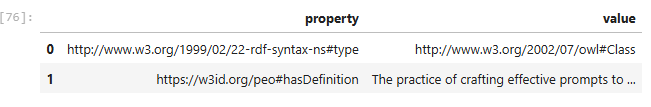
\includegraphics[width=0.9\linewidth]{Figures/fig_69.png}
    \caption{CQ1 SPARQL query results - PEO updated}
    \label{fig:69}
\end{figure}
Fig. \ref{fig:69} shows the new output of CQ1.

The second competency question CQ2: What is a prompt? is translated
into:
\begin{lstlisting}
SELECT DISTINCT ?property ?value
WHERE {
    <https://w3id.org/peo#Prompt> ?property ?value .
}
\end{lstlisting}

\begin{figure}[H]
    \centering
    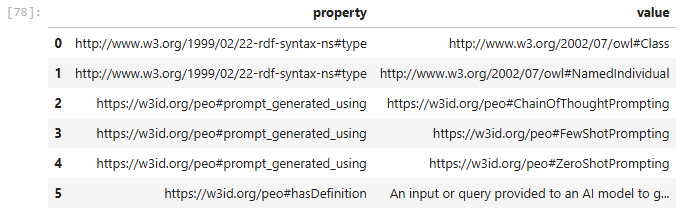
\includegraphics[width=0.9\linewidth]{Figures/fig_70.png}
    \caption{CQ2 SPARQL query results - PEO updated}
    \label{fig:70}
\end{figure}
Fig. \ref{fig:70} shows the new output of CQ2.

The third competency question CQ3: What are prompting techniques?
is translated into:
\begin{lstlisting}
SELECT DISTINCT ?instance
WHERE {
  ?instance <http://www.w3.org/1999/02/22-rdf-syntax-ns#type> <https://w3id.org/peo#PromptingTechnique> .
}
\end{lstlisting}


\begin{figure}[H]
    \centering
    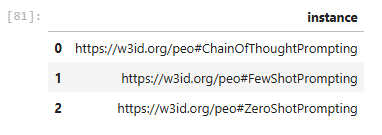
\includegraphics[width=0.7\linewidth]{Figures/fig_71.png}
    \caption{CQ3 SPARQL query results - PEO updated}
    \label{fig:71}
\end{figure}
Fig. \ref{fig:71} shows the new output of CQ3.

The ninth competency question CQ9: What are possible tasks? is translated into:
\begin{lstlisting}
SELECT DISTINCT ?instance
WHERE {
  ?instance <http://www.w3.org/1999/02/22-rdf-syntax-ns#type> <https://w3id.org/peo#Task> .
}
\end{lstlisting}

\begin{figure}[H]
    \centering
    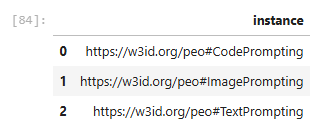
\includegraphics[width=0.6\linewidth]{Figures/fig_72.png}
    \caption{CQ9 SPARQL query results - PEO updated}
    \label{fig:72}
\end{figure}

Fig. \ref{fig:72} shows the new output of CQ9.


\section{Publication}
\label{section:5_5_publication}
The last step after the Ontology implementation in the LOT methodology is the Ontology publication phase, which scope is to provide an online ontology accessible both as human-readable documentation and a machine-readable documentation from its URI.
This phase is divided into three sub-activities:
\begin{enumerate}
    \item Propose release candidate
    \item Ontology documentation
    \item Online publication
\end{enumerate}
as we can see in the figure below:
\begin{figure}[H]
    \centering
    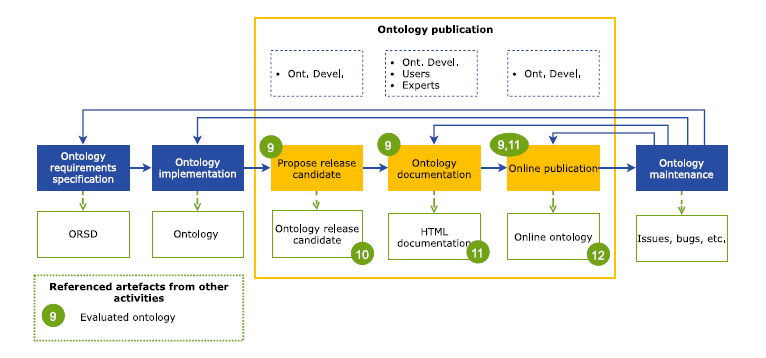
\includegraphics[width=0.9\linewidth]{Figures/fig_25.png}
    \caption{Ontology publication workflow}
    \label{fig:enter-label}
\end{figure}

\subsection{Propose Release Candidate}
\label{subsection:4_5_1_release}
After all the implementation and evaluation, in this step there is the decision about which version of the ontology is going to be published.
It is a quite easy choice because, as said in pervious sections, the version populated automatically did not add any useful information from the original version.
Moreover it added, according the OOPS! report, more pitfalls (five vs three).
\subsection{Ontology Documentation}
\label{subsection:4_5_2_docs}
The ontology documentation is generated using Protegé and the OWLdoc plug-in, which automatically generate HTML documentation starting from ontology code.
The output of OWLdoc is the following:
\begin{figure}[H]
    \centering
    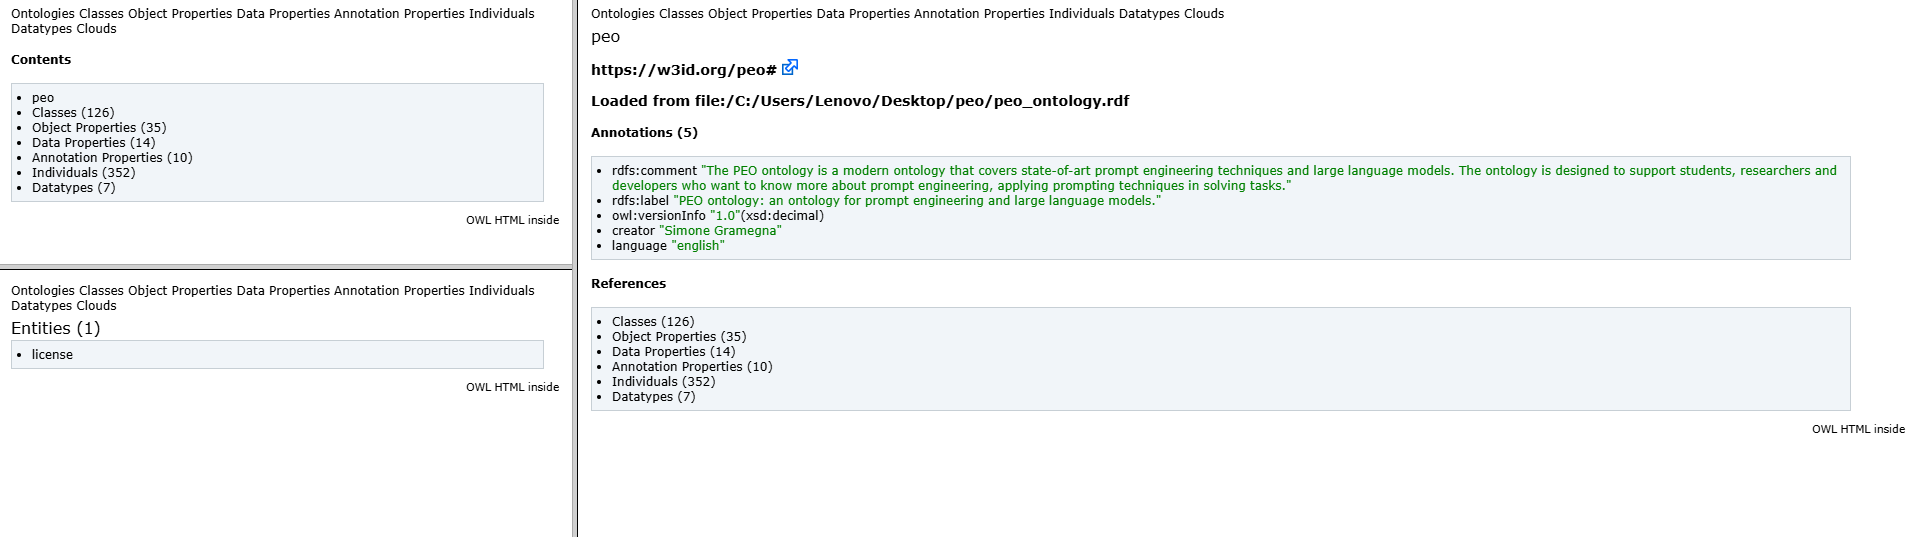
\includegraphics[width=0.9\linewidth]{Figures/fig_63.png}
    \caption{OWLdoc output}
    \label{fig:enter-label}
\end{figure}
The OWLdoc is available in the GitHub repository here \footnote{https://github.com/simonegramegna/peo/tree/main/docs} in the /docs folder and it can be consulted online here \footnote{https://peoontology.vercel.app/}
The documentation is made accessible for everyone using Vercel: a cloud platform for hosting web applications and static sites.
This free service using an integrated Github action, takes as input the documentation in the repository and publishes online automatically without requiring any effort by the developer.
The official documentation website is:
\href{https://peoontology.vercel.app/}{https://peoontology.vercel.app/}.

\subsection{Online Publication}
\label{subsection:4_5_3_publication}
Once the ontology documentation is ready, the ontology can be published online on major vocabularies repository, by accessing the ontology using its URI. I will consider two most known repositories for ontology publishing: \href{https://w3id.org/}{w3id.org} and \href{https://bioportal.bioontology.org/}{BioPortal}.

W3id.org a permanent identifier service that provides stable, persistent, and HTTP-resolvable URIs for web resource. The creation of a new identifier for publishing a new ontology is made using Github and the official W3id.org Github repository. The procedure followed is straightforward, first we fork the W3id.org Github repository on my Github, creating a "copy" of the repository. 
\begin{figure}[H]
    \centering
    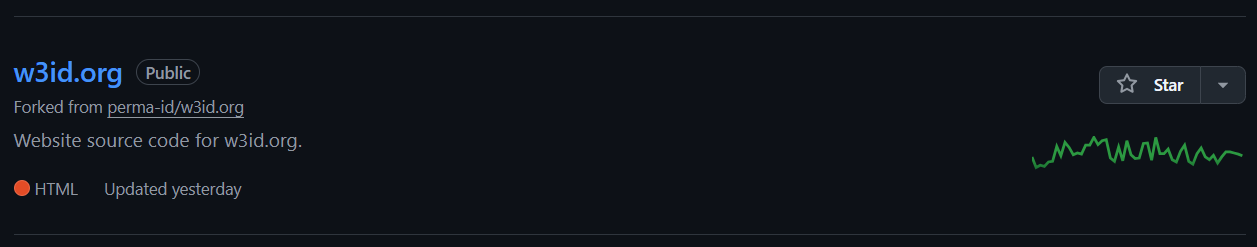
\includegraphics[width=0.9\linewidth]{Figures/fig_65.png}
    \caption{Forked W3id.org repository}
    \label{fig:enter-label}
\end{figure}
Then we create a new branch and we create a new directory with the intended permanent identifier name, in my case we create a directory called "peo". Inside this directory we create two files:
\begin{itemize}
    \item README.md: contains more identifier info and contact info, for human to read.
    \item .htaccess: contains redirection rules, for computer to read and perform.
\end{itemize}
In the case of PEO, the README.md contains all my contact information with the link to the PEO Github repository while the .htaccess contains the following redirections rules:
\begin{lstlisting}
# Activates Rewrite Engine
RewriteEngine On

# Content negotiation for RDF/XML
RewriteCond %{HTTP_ACCEPT} application/rdf\+xml
RewriteRule ^$ https://raw.githubusercontent.com/simonegramegna/peo/refs/heads/main/peo_ontology.rdf [R=303,L]

# Content negotiation for Turtle
RewriteCond %{HTTP_ACCEPT} text/turtle
RewriteRule ^$ https://raw.githubusercontent.com/simonegramegna/peo/refs/heads/main/peo_ontology.ttl [R=303,L]

# Default: serves HTML for browser or client not RDF-aware
RewriteRule ^$ https://peoontology.vercel.app/ [R=303,L]

# Blocks directory indexing
Options -Indexes
\end{lstlisting}
Once the two files are completed, we submitted a pull request to the main branch that is approved by one of repository administrators. As soon the merge of the created branch, it is possible to access to the ontology using its URI, in the case of PEO the URI is: \href{https://w3id.org/peo}{https://w3id.org/peo} bringing the user with an HTTP request to the online ontology documentation.
\begin{figure}[H]
    \centering
    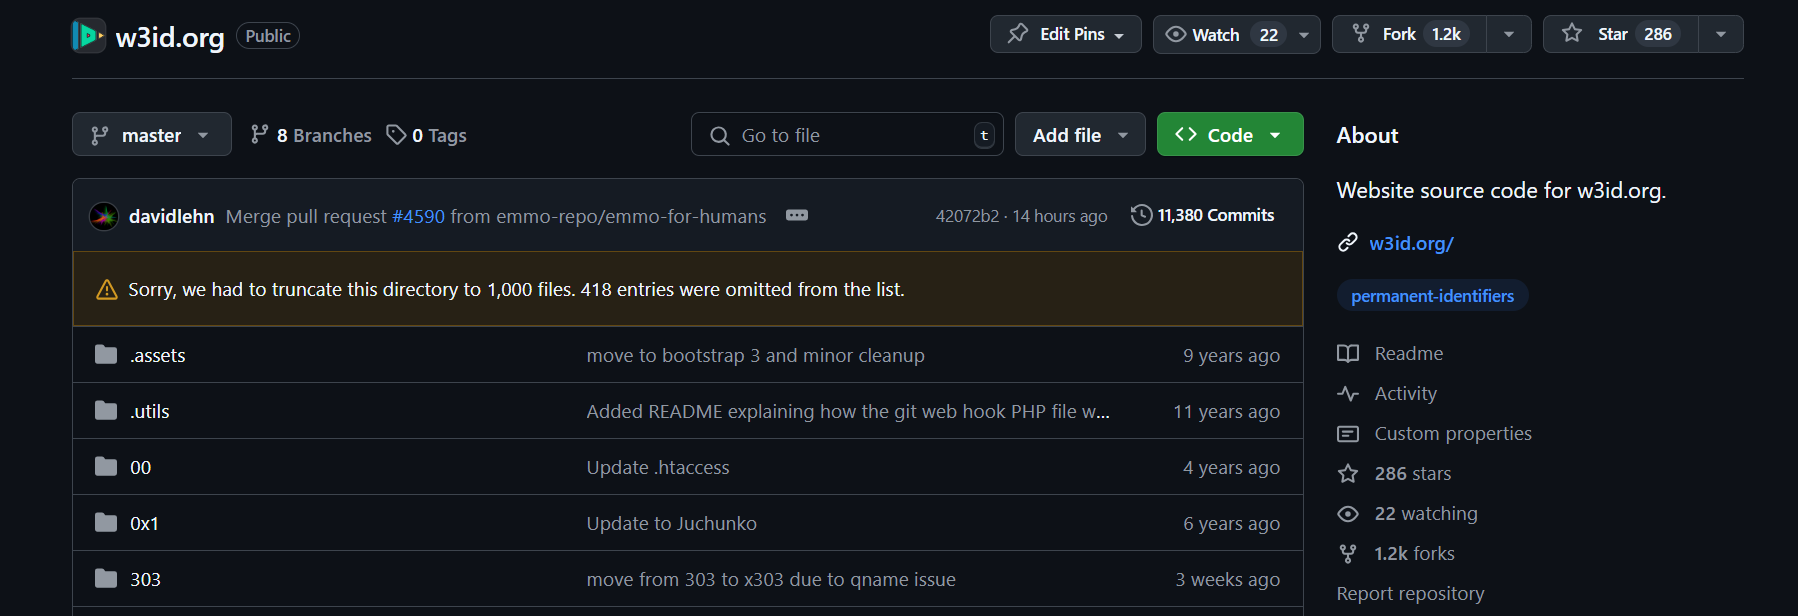
\includegraphics[width=0.9\linewidth]{Figures/fig_66.png}
    \caption{W3id.org repository main directory}
    \label{fig:66}
\end{figure}
Fig. \ref{fig:66} shows W3id.org repository main directory

We decided to publish PEO also on BioPortal\footnote{https://bioportal.bioontology.org/
}. First we create an account on BioPortal and then we specify all the informations about the ontology: the version, the type (RDF) and the release date.
\begin{figure}[H]
    \centering
    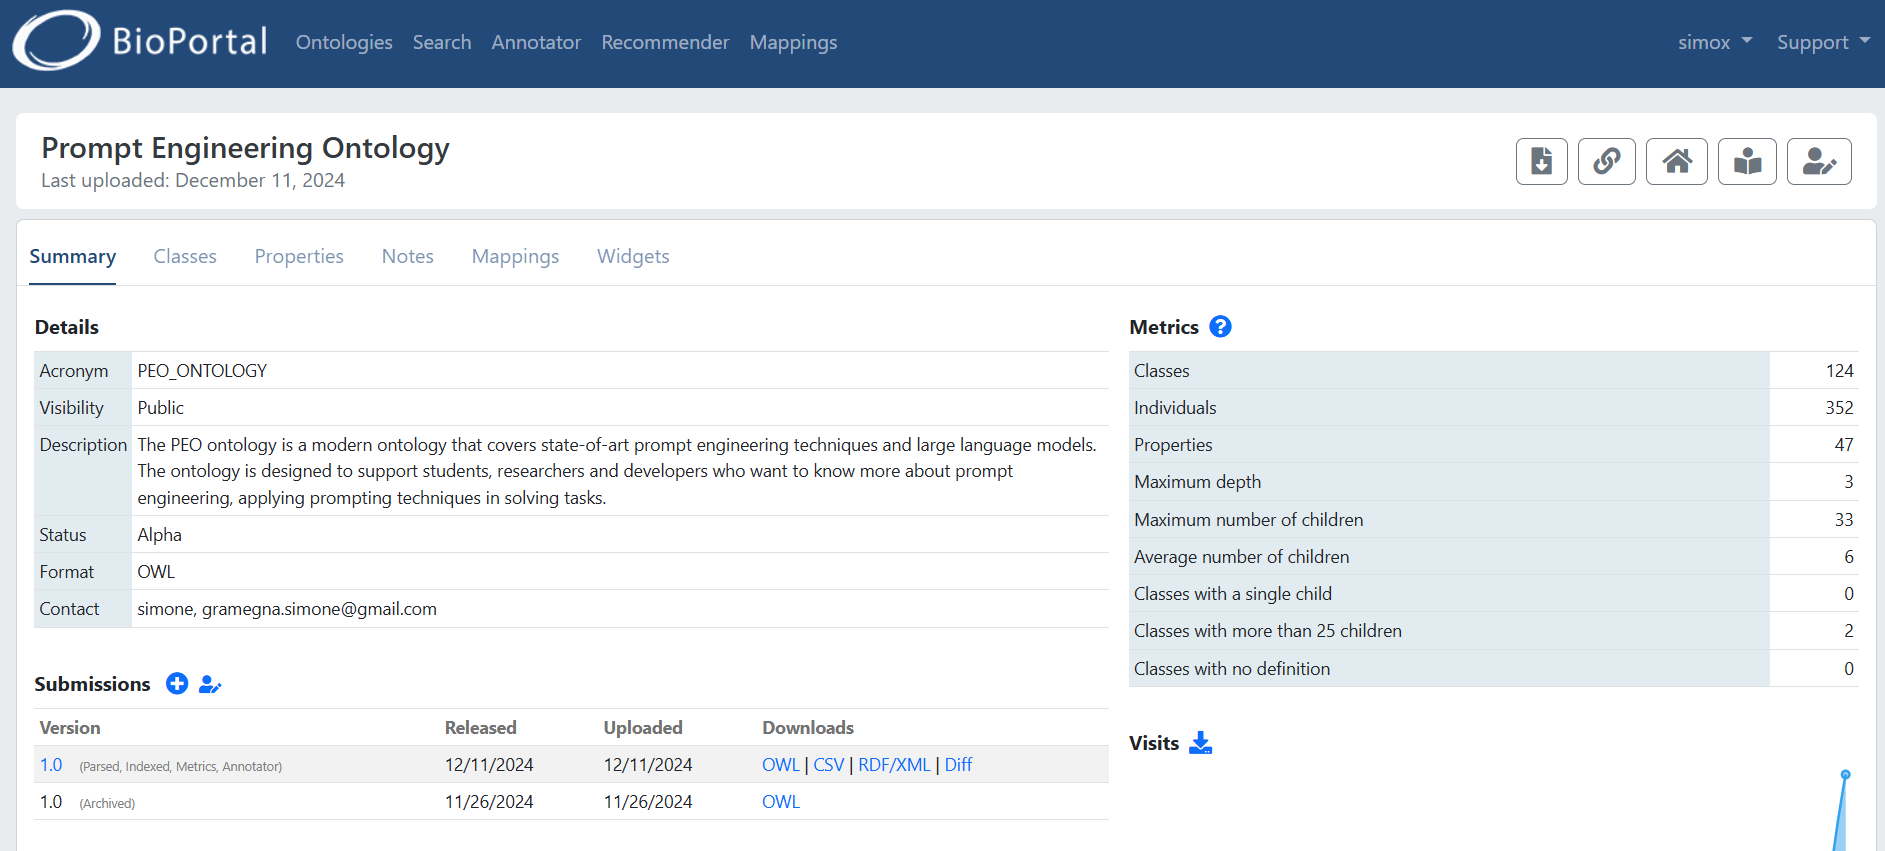
\includegraphics[width=0.9\linewidth]{Figures/fig_67.png}
    \caption{BioPortal main page}
    \label{fig:enter-label}
\end{figure}
The ontology is published here \footnote{https://bioportal.bioontology.org/ontologies/PEO_ONTOLOGY?p=summary} and it is possible using the web interface view the whole ontology: classes, object properties, data properties and individuals. This is a very useful feature because the user has no need to download any additional software, moreover BioPortal computes automatically base ontology metrics. 
\begin{figure}[H]
    \centering
    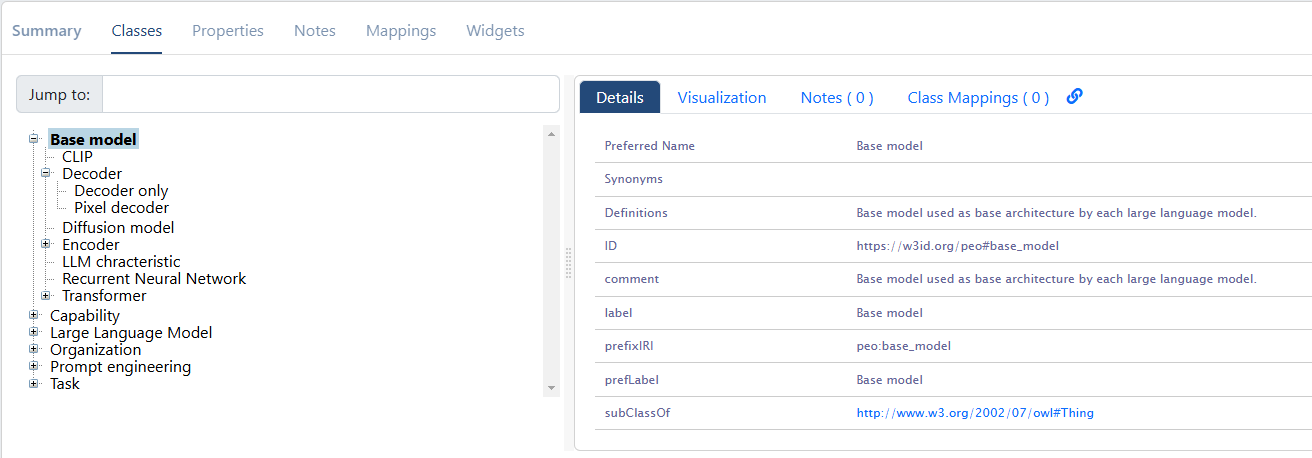
\includegraphics[width=0.9\linewidth]{Figures/fig_68.png}
    \caption{BioPortal ontology interface}
    \label{fig:enter-label}
\end{figure}


\newpage
\section{Results Discussion}
\label{section:5_6_discussion}
The design and implementation phases led the creation of an ontology that is the very first to comprehensively and exhaustively represent prompt engineering techniques and large language models.
As discussed in previous chapters, resources on these topics are often quite limited and fragmented.
So PEO becomes an important reference in these fields providing users with a useful and effective. PEO also supports developers and researchers in choosing the best prompt engineering techniques and LLM for their scopes. Additionally, it assists content creators and copywriters in selecting the most suitable approach and model for automatic content creation.

The results obtained during the evaluation process of PEO reveal important insights into its design, structure, and functionality.
Through a combination of tools and methods, such as HermiT reasoner, OntoMetrics, and OOPS! validation, the ontology was rigorously assessed, highlighting both its strengths and areas for improvement.

There are three main strengths of the PEO found during the evaluation:
\begin{enumerate}
    \item Logical Consistency and Reasoning: the HermiT reasoner confirmed that the ontology's logical structure is sound, with no inconsistencies detected in both the manually populated version and the updated version generated by GPT-4. Moreover, additional triples and axioms are inferred. 

    \item Expressiveness and Structural Metrics: OntoMetrics demonstrated the ontology’s comprehensiveness, with 2684 axioms and $SRIF(D)$ expressivity, supporting advanced reasoning while maintaining computational efficiency. The hierarchical organization (199 SubClassOf axioms) facilitates inheritance.
    Moreover, the inclusion of 352 individuals indicates practical applicability.

    \item Semantic Coverage: competency questions translated into SPARQL queries yielded the expected results, confirming that the ontology effectively represents key concepts, such as prompting techniques, tasks, and the relationships between prompts and their generated responses. This shows that the ontology is well-aligned with its design goals.
\end{enumerate}

The evaluation found also the following limitations:
\begin{itemize}
    \item Pitfalls in Structure: OOPS! detected structural
    issues, such as unconnected elements and missing annotations. These issues were more 
    in the GPT-4-populated version, where newly introduced classes (e.g., Task, PromptingTechnique) lacked connections to the broader ontology. This indicates that automated population requires further refinement.

    \item Simplistic Relationships: metrics such as low relationship richness (0.160338) suggest that the ontology is more focused on defining concepts than on establishing interconnections. While this simplifies reasoning, it may limit the representation of complex semantic relationships.

    \item Underutilized Properties: object and data property axioms reveal limited use of features such as functional, symmetric, or inverse properties. Incorporating these could enhance the ontology's ability to model constraints and unique relationships.

    \item Inconsistencies in Naming Conventions: the naming conventions of new classes in the other version of PEO introduced by GPT-4 deviated from the original ontology’s standards, potentially affecting usability and integration.
\end{itemize}
In general, the major issues are present in the version of the PEO populated using GPT-4, as, as previously observed, it has not proven capable of correctly populating the original version of the ontology with new instances. Regarding the original version of the PEO, there are solvable pitfalls, which I will discuss in the next section.


Considering the limitations outlined in the previous section, caused by the pitfalls in the main version of the PEO, we proceed to address and correct the identified pitfalls:
\begin{itemize}
    \item P04 - Creating unconnected ontology elements: this pitfall involves the prompt\_engineering class which has no relation with any other class in the ontology.

    \item P34 - Untyped class: this pitfall involves elements in SWRL rules.

    \item P41 - No license declared: this pitfall is due to the absence of the license in the ontology.
\end{itemize}
The resolution of these pitfalls is essential to enhance the quality of the published ontology.

The pitfall P04, as said before, involves the prompt\_engineering class which has no relation with any other class in the ontology, this because the prompt\_engineering is a sort of "container" of classes related to prompt. In order to connect prompt\_engineering we created the object property applied\_to (with inverse relation supports) which connects prompt\_engineering with the large\_language\_model class.

\begin{figure}[H]
    \centering
    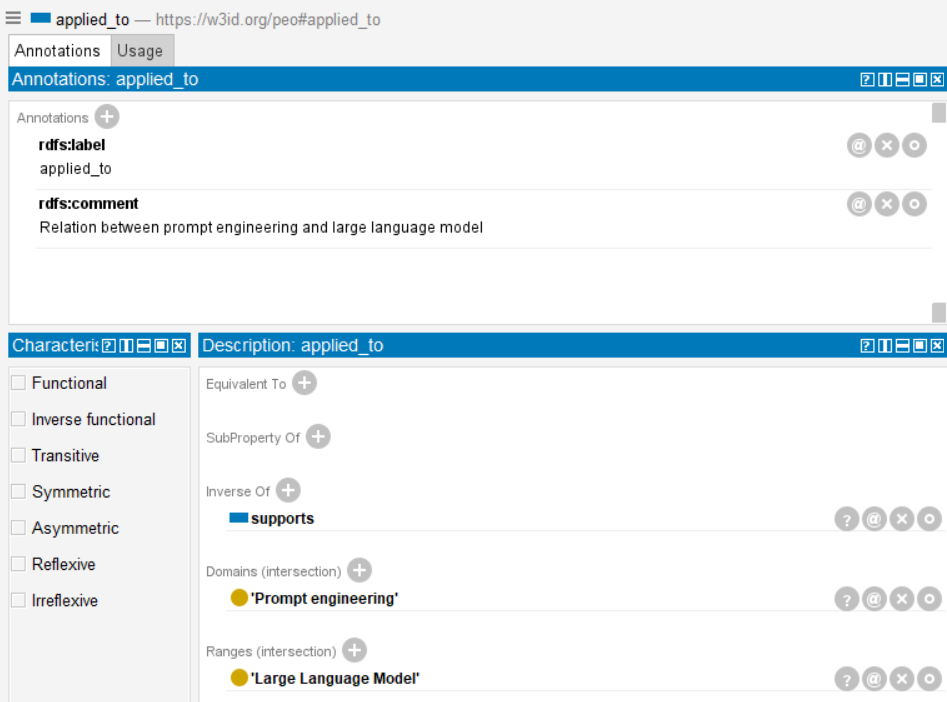
\includegraphics[width=0.7\linewidth]{Figures/fig_78.png}
    \caption{Object property between Prompt Engineering class and Large Language Model class}
    \label{fig:enter-label}
\end{figure}

The pitfall P34 stems from constructs automatically created by Protegé when a SWRL rule is defined.
In fact, SWRL is not part of the OWL languages so the types of the variables are not recognized.
To address this issue, we removed the SWRL rules and replaced them with property chains defined in OWL.
In this way, it is possible not only to reduce complexity, as SWRL rules involve a non-negligible computational cost, but also to make the ontology more portable, given that not all reasoners support SWRL rules.\\
In this case, we replaced the SWRL rule:
\begin{lstlisting}
peo:develops(?c, ?x) ^ peo:has_variant(?x, ?y) -> peo:develops(?c, ?y)
\end{lstlisting}
with the following object property chain:
\begin{figure}[H]
    \centering
    
\includegraphics[width=0.7\linewidth]{Figures/fig_81.png}
    \caption{Object property chaining for develops}
    \label{fig:enter-label}
\end{figure}
The same approach is applied to the other object properties. A particular case is the SWRL rule S2: 
\begin{lstlisting}
peo:evolves(?x, ?y) -> peo:has_variant(?x, ?y)
\end{lstlisting}
In which, instead of using the property chain, we define it directly as an object property evolves as sub property of has\_variant as we can see in the figure below:
\begin{figure}[H]
    \centering
    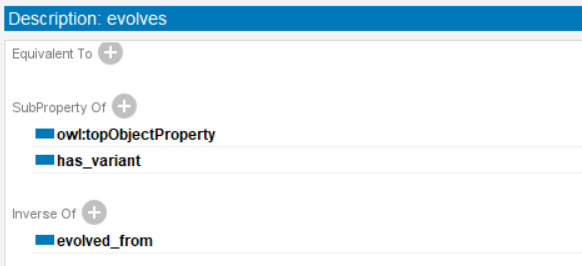
\includegraphics[width=0.9\linewidth]{Figures/fig_82.png}
    \caption{evolves object property}
    \label{fig:enter-label}
\end{figure}
When the HermiT reasoner is activated, the inferences derived from the property chains are equivalent to those produced by the SWRL rules.

The pitfall P41, as said before, is due to the absence of the license in the ontology.
In order to solve this pitfall, I added the annotation property dcterms:license  as in \cite{yusof2019malaysian} with the link of the license (GNU General Public License v3) as value. Fig. \ref{fig:79} as we can see in the figure below:
\begin{figure}[H]
    \centering
    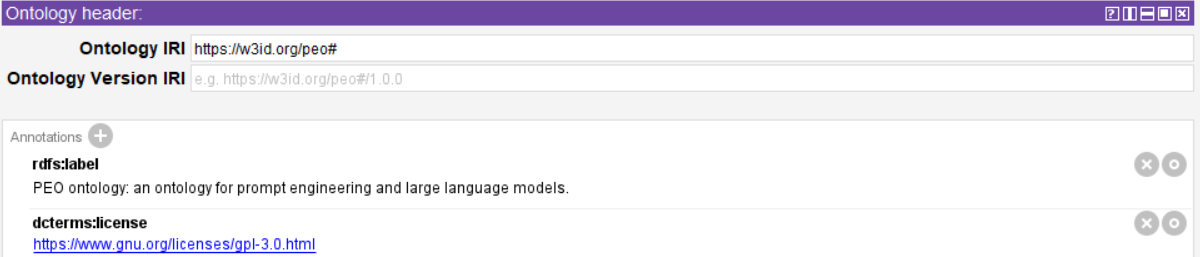
\includegraphics[width=0.9\linewidth]{Figures/fig_79.png}
    \caption{License annotation in PEO}
    \label{fig:79}
\end{figure}
To solve this pitfall, instead of using software license like GNU General Public License, I used the Creative Commons license available at this link: \href{https://creativecommons.org/licenses/by/4.0/}{https://creativecommons.org/licenses/by/4.0/}.

During the revision phase, it has been noted that class, object properties and data properties name do not follow the Semantic Web naming conventions that establishes Camel Case for class names, with the first letter in upper case while for object properties and data properties the Camel Case is used but the first letter is in lower case.
For example the object property evolved\_from with this modification, it becomes evolvedFrom and the large\_language\_model class becomes LargeLanguageModel.


We stated two RQs in Chapter:
\begin{enumerate}
      \item RQ~1: Does PEO provide comprehensive and consistent knowledge on LLMs and prompt engineering?

    \item RQ~2: Can we use PEO to infer additional knowledge?
\end{enumerate}

At the end of the experimental evaluation, it is possible to give an answer to the RQs.
The answer to RQ 1, is: yes.
Based on the results obtained during the testing and evaluation phase, we can say that PEO provides comprehensive and consistent knowledge on LLMs and prompt engineering. The execution of SPARQL queries confirms that PEO is able to provide correct informations on concepts like prompt, prompting technique, large language models and task. From the analysis of the results obtained with OntoMetrics, PEO has a good number of classes (126) and individuals (352), with individuals interconnected through 34 object properties. The tangledness equal to 0.26 and the relationships richness equal to 0.16 demonstrates that PEO is not complex and it has moderate relations between concepts.

Also the answer to RQ 2 is: yes.
The inference mechanism and property chaining defined in the PEO makes possible to get informations about all the characteristics of each large language model represented and the connections with prompts generated using prompt engineering techniques. Minor issues highlighted by pitfalls have been resolved once identified, ensuring the quality of the final result.


Despite these minor issues, the PEO is well-designed, comprehensive, well-documented, and has very few problems.
It significantly outperforms state-of-the-art ontologies related to large language models and prompt engineering.